\documentclass{standalone}
\usepackage{amsfonts, amsmath, amssymb, bm} %Math fonts and symbols
\usepackage{dcolumn, multirow} % decimal-aligned columns, multi-row cells
\usepackage[colorlinks=true]{hyperref}
\usepackage{graphicx, subfigure, float} % graphics commands
\usepackage[margin=1in]{geometry} % sets page layout
\usepackage{setspace}% allows toggling of double/single-spacing
\usepackage{verbatim}% defines environment for un-evaluated code
\usepackage{natbib}% defines citation commands and environments.
\singlespace % set document spacing to single
\bibpunct[, ]{(}{)}{,}{a}{}{,} % sets the punctuation of the bibliography entires.
\newcolumntype{d}[1]{D{.}{.}{#1}} % defines a decimal-aligned column
\usepackage{tikz}
\usetikzlibrary{intersections}
\usepackage{enumerate}
\usepackage[utf8]{inputenc}
\usepackage[english]{babel}
\usetikzlibrary{shapes.geometric}
\hyphenpenalty=10000

\begin{document}
    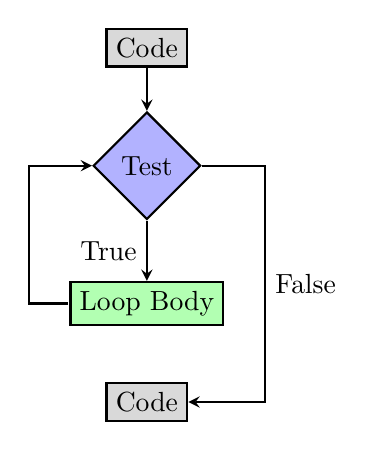
\begin{tikzpicture}[>=stealth]
        \begin{scope}
            \node [thick,rectangle, draw, fill = gray!30] (a) at (0,0) {Code}; 
            \node [thick,diamond, draw, fill = blue!30] (b) at (0,-1.5) {Test};
            \node [thick,rectangle, draw, fill = green!30] (c) at (0, -3.25) {Loop Body};
            \node [thick,rectangle, draw, fill = gray!30] (e) at (0,-4.5) {Code};
            \draw [->, thick] (a) -- (b);
            \draw [thick, ->] (.7,-1.5) -- (1.5,-1.5) -- node [right] {False} (1.5, -4.5) -- (e);
            \draw [->, thick] (b) -- node [left] {True} (c);
            \draw [->, thick] (-1,-3.25) -- (-1.5, -3.25) -- (-1.5, -1.5) -- (b);
        \end{scope}
        
    \end{tikzpicture}
\end{document}
